% !TEX program = pdflatex
% CEB-ViTAL manuscript. Compile: pdflatex -> bibtex -> pdflatex -> pdflatex
% (LaTeX Workshop recipe in .vscode/settings.json; on Overleaf upload the folder as a zip).
% All result numbers come from numbers.tex and tables/*.tex, generated by
% ../paper/make_latex_assets.py from the simulation data. Do not type results by hand.
\documentclass[journal]{IEEEtran}

\usepackage{cite}
\usepackage{amsmath,amssymb}
\usepackage{graphicx}
\usepackage{booktabs}
\usepackage{xcolor}
\usepackage{url}
\usepackage{tikz}
\usetikzlibrary{arrows.meta,positioning,fit}
\IfFileExists{algorithm.sty}{\usepackage{algorithm}}{%
  \usepackage{float}\newfloat{algorithm}{tbp}{loa}\floatname{algorithm}{Algorithm}}
\usepackage{algpseudocode}
\usepackage[hidelinks]{hyperref}
\hypersetup{pdftitle={CEB-ViTAL: Coverage-Aware, Energy-Balanced Clustering for Lifetime Extension in Wireless Sensor Networks}, pdfauthor={Ali Hamza, Javed Iqbal}}

% Auto-generated by paper/make_latex_assets.py from results/*.json. Do not edit by hand.
\newcommand{\NRuns}{6{,}900}
\newcommand{\NRob}{1{,}080}
\newcommand{\NFair}{7{,}620}
\newcommand{\TninetyBest}{+21\% to +130\%}
\newcommand{\FNDLeach}{+40\% to +184\%}
\newcommand{\FNDDeec}{+28\% to +151\%}
\newcommand{\FNDVital}{+224\% to +2519\%}
\newcommand{\CovBest}{+15\% to +148\%}
\newcommand{\ReadAll}{$-$4\% to +1\%}
\newcommand{\SthreeTninety}{+2\% to +17\%}
\newcommand{\CzeroSthree}{19\%}
\newcommand{\CzeroSoneHundred}{56\%}
\newcommand{\CzeroSoneFive}{92\%}
\newcommand{\AblMone}{93--97\%}
\newcommand{\LNDcebH}{7294}
\newcommand{\LNDleachH}{8954}
\newcommand{\LNDvitalH}{11376}
\newcommand{\LNDcebF}{16415}
\newcommand{\LNDmaxF}{11696}
\newcommand{\TcebThree}{10686}
\newcommand{\TbestThree}{5758}
\newcommand{\MthreeSthree}{0\% to +3\%}
\newcommand{\LeachCovSone}{+23\% to +61\%}
\newcommand{\RobSoneFone}{+10\% to +56\%}
\newcommand{\RobSthreeFone}{$-$3\% to +6\%}
\newcommand{\PMax}{6.1\times10^{-6}}

% Auto-generated by paper/make_extra_figures.py. Do not edit by hand.
\newcommand{\SnapRound}{5500}
\newcommand{\SnapN}{300}
\newcommand{\SnapLeachAlive}{230}
\newcommand{\SnapLeachSensing}{230}
\newcommand{\SnapLeachCov}{77\%}
\newcommand{\SnapLeachE}{0.05}
\newcommand{\SnapVitalAlive}{163}
\newcommand{\SnapVitalSensing}{163}
\newcommand{\SnapVitalCov}{67\%}
\newcommand{\SnapVitalE}{0.15}
\newcommand{\SnapEbAlive}{300}
\newcommand{\SnapEbSensing}{300}
\newcommand{\SnapEbCov}{85\%}
\newcommand{\SnapEbE}{0.03}
\newcommand{\SnapCebAlive}{300}
\newcommand{\SnapCebSensing}{144}
\newcommand{\SnapCebCov}{81\%}
\newcommand{\SnapCebE}{0.27}
\newcommand{\SensCeb}{148}
\newcommand{\SensEb}{300}
\newcommand{\HeatMin}{+2\%}
\newcommand{\HeatMax}{+140\%}

\newcommand{\todo}[1]{\textcolor{red}{[#1]}}
\newcommand{\TN}{T_{90}}

\begin{document}

\title{CEB-ViTAL: Coverage-Aware, Energy-Balanced Clustering for Lifetime Extension in Wireless Sensor Networks}

\author{Ali~Hamza and Javed~Iqbal%
\thanks{A. Hamza is with \todo{Department, Institution, City, Country} (e-mail: \todo{e-mail}).}%
\thanks{J. Iqbal is with the Department of Computer Software Engineering, National University of Sciences and Technology (NUST), Islamabad 44000, Pakistan (e-mail: \todo{e-mail}).}%
\thanks{Corresponding author: \todo{name}.}}

\markboth{\todo{Journal name}}{Hamza and Iqbal: CEB-ViTAL}

\maketitle

\begin{abstract}
ViTAL is a recent three-phase lifetime-extension approach for wireless sensor networks (WSNs). It combines harmony-search deployment for coverage, a connected dominating set (CDS), and a four-factor cluster-head (CH) score. We show that its CH score is almost insensitive to residual energy, favours CHs far from the sink, and concentrates the CH role on a small CDS backbone. We also note that coverage, although optimised at deployment, is ignored during operation.

We propose CEB-ViTAL, which keeps ViTAL's deployment phase and adds three mechanisms:
(i) a coverage-preserving, energy-weighted sleep scheduler;
(ii) a normalised four-factor score with a dynamic energy weight, used to elect the analytically optimal number of spatially separated CHs;
(iii) energy-aware multi-hop forwarding from CHs to the sink.

All protocols were evaluated in one shared simulator over \NRuns{} runs on 30 held-out random networks, six scenarios and 100--500 nodes. Hypotheses and constants were pre-registered.

In the base setting of ViTAL (100\,m field, corner sink), CEB-ViTAL extends the 90\% coverage lifetime by \TninetyBest{} over the strongest baseline. It extends first-node death by \FNDLeach{} over LEACH and \FNDVital{} over ViTAL, and the coverage integral by \CovBest{}. Every pre-registered test is significant (Holm-corrected $p\le\PMax$). Readings delivered differ by \ReadAll{} from always-on protocols. Gains shrink in sparse deployments. In the base setting they remain positive even when sleeping is charged as much as transmitting.
\end{abstract}

\begin{IEEEkeywords}
Wireless sensor networks, clustering, LEACH, coverage preservation, sleep scheduling, energy balance, network lifetime.
\end{IEEEkeywords}

\section{Introduction}
\IEEEPARstart{W}{ireless} sensor networks (WSNs) support environmental monitoring, health care, smart homes and industrial IoT~\cite{akyildiz2002survey}. Their nodes run on batteries that are rarely replaced, so energy efficiency decides how long a deployment can serve its purpose.

Hierarchical clustering, introduced by LEACH~\cite{heinzelman2000leach,heinzelman2002leachc}, rotates the cluster-head (CH) role so that the high cost of long-range transmission is shared. Many successors refine the CH election with energy, distance and topology information~\cite{smaragdakis2004sep,younis2004heed,qing2006deec,mohamed2026clustering}.

ViTAL~\cite{ali2025vital} argues that deployment, topology and radio conditions must be treated together. It has three phases:
\begin{itemize}
\item a harmony-search (HSA) deployment that maximises coverage~\cite{geem2001harmony,alia2017hsa};
\item a connected-dominating-set (CDS) backbone~\cite{guha1998cds};
\item a four-factor (4F) CH score built from residual energy, neighbour count, distance to the sink and signal-to-noise ratio (SNR).
\end{itemize}
ViTAL reports large gains over LEACH and two of its variants, and names dynamic weighting and scheduling as future work.

This paper continues that line of work. Re-implementing ViTAL from its description, we found three weaknesses in how its CH score is normalised and applied. We also note a missed opportunity: the coverage that phase~1 optimises is never used during operation, so every node senses and reports every round even where its area is already covered.

\textbf{Contributions.}
\begin{enumerate}
\item An analysis of ViTAL's CH selection. Its energy term scales as $1/N$, its distance term favours far nodes, and its CDS restriction concentrates load (Section~\ref{sec:analysis}).
\item CEB-ViTAL. The protocol couples ViTAL's coverage-driven deployment with coverage-preserving, energy-weighted sleep scheduling and a corrected, energy-balanced clustering phase (Section~\ref{sec:method}).
\item A pre-registered evaluation on held-out random networks against LEACH, DEEC, ViTAL and our intermediate design EB-ViTAL. It covers six scenarios, includes ablations and a sleep-energy robustness check, and uses paired non-parametric tests with multiplicity control (Sections~\ref{sec:setup}--\ref{sec:results}).
\end{enumerate}

\section{Related Work}\label{sec:related}
\todo{Authors: extend this section with a systematic 2023--2026 literature search on coverage-preserving clustering and duty cycling before submission.}

\textbf{Clustering protocols.}
\begin{itemize}
\item LEACH~\cite{heinzelman2000leach} elects CHs at random, with probability $p$ and an epoch-based rotation.
\item LEACH-C~\cite{heinzelman2002leachc} centralises the election at the sink and derives the optimal number of clusters.
\item SEP~\cite{smaragdakis2004sep} and DEEC~\cite{qing2006deec} weight the CH probability by initial or residual energy relative to the network average.
\item HEED~\cite{younis2004heed} combines residual energy with a communication cost and a competition range that spreads CHs.
\item PEGASIS~\cite{lindsey2002pegasis} replaces clusters with a chain.
\item Multi-hop LEACH variants such as EEM-LEACH~\cite{antoo2014eemleach} relay CH traffic to avoid long single-hop links.
\end{itemize}

\textbf{Coverage-preserving scheduling.} When nodes are deployed densely, their sensing areas overlap, and redundant nodes can sleep without losing coverage.
\begin{itemize}
\item Slijepcevic and Potkonjak~\cite{slijepcevic2001power} and Cardei and Du~\cite{cardei2005setcover} organise nodes into covering sets that are activated in turn.
\item Tian and Georganas~\cite{tian2002coverage} let each node decide locally whether its area is already covered by neighbours.
\item CCP~\cite{wang2003ccp} and OGDC~\cite{zhang2005ogdc} jointly maintain coverage and connectivity.
\item Randomised independent sleeping~\cite{kumar2004kcoverage} provides analytical coverage guarantees.
\item Soro and Heinzelman~\cite{soro2009coverage} make CH selection itself coverage-aware.
\item Greedy weighted set cover~\cite{chvatal1979greedy} is the standard approximation for choosing a covering subset.
\end{itemize}

\textbf{ViTAL~\cite{ali2025vital}.} It integrates HSA deployment, a CDS and 4F CH selection. The present work keeps its deployment phase, replaces its CDS-restricted 4F election, and adds coverage-preserving scheduling. Combining coverage scheduling with corrected, energy-balanced clustering on top of a coverage-optimised deployment is the contribution claimed here.

\section{System Model}\label{sec:model}
\subsection{Network and energy model}
$N$ static sensors are deployed in an $M\times M$ field. The sink is either static or follows a random-waypoint path. Every node starts with energy $E_0$. In each round, every \emph{sensing} node produces one $L$-bit reading. Members send their readings to a CH, which aggregates them and forwards one packet towards the sink.

We use the first-order radio model~\cite{heinzelman2002leachc}:
\begin{equation}
E_{\mathrm{TX}}(L,d)=\begin{cases}L E_{\mathrm{elec}}+L\varepsilon_{\mathrm{fs}}d^{2}, & d<d_0,\\ L E_{\mathrm{elec}}+L\varepsilon_{\mathrm{mp}}d^{4}, & d\ge d_0,\end{cases}
\end{equation}
with $E_{\mathrm{RX}}(L)=L E_{\mathrm{elec}}$ and $d_0=\sqrt{\varepsilon_{\mathrm{fs}}/\varepsilon_{\mathrm{mp}}}$. Aggregation costs $E_{\mathrm{DA}}$ per bit per signal. Table~\ref{tab:params} lists all parameters.

\subsection{Coverage model and metrics}
As in ViTAL, the field is divided into $1\,$m demand cells, and node $i$ covers cell $c$ if $\lVert \mathbf{p}_c-\mathbf{x}_i\rVert\le R_s$. Let $\mathcal{A}(r)$ be the set of sensing nodes in round $r$ and $\mathcal{C}_i$ the cells covered by node $i$. The covered fraction is
\begin{equation}
C(r)=\frac{1}{M^2}\Bigl|\bigcup_{i\in\mathcal{A}(r)}\mathcal{C}_i\Bigr|,
\end{equation}
and $C_0$ is the value of $C(0)$ with all nodes active.
The primary metric is the \emph{coverage lifetime}
\begin{equation}
\TN=\min\{r: C(r)<0.9\,C_0\}.
\end{equation}

We also report:
\begin{itemize}
\item the coverage integral $\sum_r C(r)$, in coverage-rounds;
\item first, half and last node death (FND, HND, LND);
\item the number of readings delivered to the sink.
\end{itemize}

\begin{table}[t]
\caption{Simulation Parameters}\label{tab:params}
\centering\scriptsize
\setlength{\tabcolsep}{4pt}
\begin{tabular}{ll}
\toprule
Parameter & Value\\
\midrule
Field size $M$ & 100\,m (S1, S2, S5, S6), 200\,m (S3, S4)\\
Nodes $N$ & 100, 200, 300, 400, 500\\
Initial energy $E_0$ & 0.5\,J\\
$E_{\mathrm{elec}}$, $E_{\mathrm{DA}}$ & 50\,nJ/bit, 5\,nJ/bit/signal\\
$\varepsilon_{\mathrm{fs}}$, $\varepsilon_{\mathrm{mp}}$ & 10\,pJ/bit/m$^2$, 0.0013\,pJ/bit/m$^4$\\
Packet size $L$ & 800\,bits (4000\,bits in S6)\\
Sensing / neighbour range & $R_s=5$\,m / 15\,m\\
LEACH CH probability $p$ & 0.1\\
SNR model & $P_t$ 0\,dBm, $PL_0$ 40\,dB, $n$ 3, $\sigma$ 4\,dB, noise $-$100\,dBm\\
HSA (phase 1) & HMS 10, HMCR 0.9, PAR 0.3, BW 5, 2000 it.\\
CovSched & $\tau=0.95$, $r_s=10$, $L_{\mathrm{ctrl}}=200$\,bits\\
Seeds & 30 held-out networks (1000--1029)\\
\bottomrule
\end{tabular}
\end{table}

\section{Analysis of ViTAL's Cluster-Head Selection}\label{sec:analysis}
ViTAL elects node $n$ as CH if a uniform random number is below $\mathrm{NV}_n\cdot T(n)$. Here $T(n)$ is the LEACH threshold, and the normalisation vector is
\begin{equation}\label{eq:nv}
\mathrm{NV}_n=w_1\frac{E_{\mathrm{res}}}{E_{\mathrm{res}}^{\mathrm{total}}}+w_2\frac{\mathrm{Neigh}}{N}+w_3\frac{\mathrm{Dist}}{\overline{\mathrm{Dist}}}+w_4\frac{\mathrm{SNR}}{\overline{\mathrm{SNR}}},
\end{equation}
with $\sum w_k=1$~\cite{ali2025vital}. We identify four issues.

\textbf{G1, near energy-blindness.} The energy term divides a node's energy by the \emph{network total}, so it is approximately $1/n_{\mathrm{alive}}$. The distance and SNR terms, in contrast, are approximately $1$. At $N=100$ with equal weights, the energy term contributes about $0.0025$, against about $0.25$ for each of the other terms. Residual energy therefore barely influences the election. When a deterministic election uses \eqref{eq:nv} unchanged, the same nodes are chosen repeatedly and first-node death falls by \AblMone{} compared with our corrected score.

\textbf{G2, inverted distance preference.} $\mathrm{Dist}/\overline{\mathrm{Dist}}$ increases with distance, so the score favours CHs \emph{far} from the sink. With the sink in a corner, as in ViTAL's set-up, such CHs pay the $d^4$ amplifier cost.

\textbf{G3, CDS bottleneck.} Restricting candidates to the CDS concentrates the CH role on a backbone of about 28 nodes, whatever $N$ is. In our simulations ViTAL has the shortest FND of all protocols, and its FND falls as $N$ grows (Table~\ref{tab:s1}).

\textbf{G4, no coverage awareness.} Coverage is maximised at deployment and then ignored. In dense deployments many nodes are redundant, yet all of them spend energy every round.

\section{Proposed Method: CEB-ViTAL}\label{sec:method}
Fig.~\ref{fig:arch} summarises the three phases. Like LEACH-C and ViTAL, CEB-ViTAL is coordinated by the sink, which knows node positions and residual energies.

\begin{figure}[t]
\centering
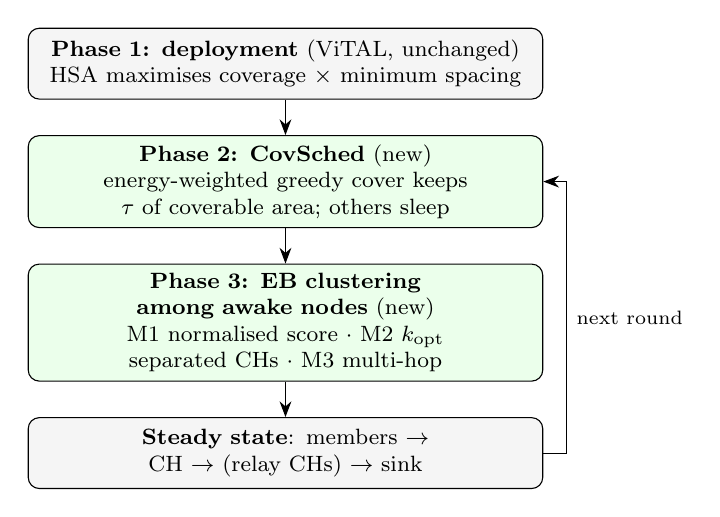
\begin{tikzpicture}[font=\footnotesize, box/.style={draw, rounded corners, align=center, text width=6.3cm, minimum height=0.9cm, fill=gray!8}, >={Stealth[length=2mm]}]
\node[box] (p1) {\textbf{Phase 1: deployment} (ViTAL, unchanged)\\ HSA maximises coverage $\times$ minimum spacing};
\node[box, below=0.45cm of p1, fill=green!8] (p2) {\textbf{Phase 2: CovSched} (new)\\ energy-weighted greedy cover keeps $\tau$ of coverable area; others sleep};
\node[box, below=0.45cm of p2, fill=green!8] (p3) {\textbf{Phase 3: EB clustering among awake nodes} (new)\\ M1 normalised score $\cdot$ M2 $k_{\mathrm{opt}}$ separated CHs $\cdot$ M3 multi-hop};
\node[box, below=0.45cm of p3] (p4) {\textbf{Steady state}: members $\to$ CH $\to$ (relay CHs) $\to$ sink};
\draw[->] (p1) -- (p2); \draw[->] (p2) -- (p3); \draw[->] (p3) -- (p4);
\draw[->] (p4.east) -- ++(0.3,0) |- node[pos=0.25, right, font=\scriptsize]{next round} (p2.east);
\end{tikzpicture}
\caption{CEB-ViTAL. Phase~1 is inherited from ViTAL~\cite{ali2025vital}; phases~2 and~3 are the contributions of this work. The active set is recomputed every $r_s$ rounds and whenever an active node dies.}\label{fig:arch}
\end{figure}

\subsection{Phase 1: coverage-driven deployment}
Phase~1 is unchanged from ViTAL~\cite{ali2025vital,alia2017hsa}. Harmony search places the $N$ nodes to maximise the coverage ratio multiplied by the normalised minimum inter-node distance, using the parameters in Table~\ref{tab:params}.

\subsection{Phase 2: coverage-preserving sleep scheduling (CovSched)}
Let $\mathcal{U}$ be the set of cells coverable by all alive nodes. Every $r_s$ rounds, and whenever an active node dies, the sink computes an active set $\mathcal{A}$ with an energy-weighted greedy set cover (Algorithm~\ref{alg:cov})~\cite{chvatal1979greedy}. Each step selects
\begin{equation}
i^\star=\arg\max_{i\notin\mathcal{A}}\ \bigl|\mathcal{C}_i\setminus \textstyle\bigcup_{j\in\mathcal{A}}\mathcal{C}_j\bigr|\cdot\frac{E_i}{\max_j E_j}
\end{equation}
until $\tau|\mathcal{U}|$ cells are covered.

Sleeping nodes neither sense nor transmit. Every alive node pays $L_{\mathrm{ctrl}}E_{\mathrm{elec}}$ per reschedule to receive the schedule. Weighting by residual energy rotates the sensing duty towards nodes with more energy. The target $\tau<1$ prevents a single node with a unique cell from being kept awake permanently.

\begin{algorithm}[t]
\caption{CovSched (run at the sink)}\label{alg:cov}
\begin{algorithmic}[1]
\Require alive set $\mathcal{L}$, energies $E$, cell sets $\mathcal{C}_i$, target $\tau$
\State $\mathcal{U}\gets\bigcup_{i\in\mathcal{L}}\mathcal{C}_i$;\; $\mathcal{A}\gets\emptyset$;\; $\mathcal{K}\gets\emptyset$
\While{$|\mathcal{K}|<\tau|\mathcal{U}|$}
  \State $i^\star\gets\arg\max_{i\in\mathcal{L}\setminus\mathcal{A}} |\mathcal{C}_i\setminus\mathcal{K}|\cdot E_i/\max_{j\in\mathcal{L}}E_j$
  \If{$|\mathcal{C}_{i^\star}\setminus\mathcal{K}|=0$} \textbf{break} \EndIf
  \State $\mathcal{A}\gets\mathcal{A}\cup\{i^\star\}$;\; $\mathcal{K}\gets\mathcal{K}\cup\mathcal{C}_{i^\star}$
\EndWhile
\State broadcast $\mathcal{A}$; nodes in $\mathcal{L}\setminus\mathcal{A}$ sleep
\end{algorithmic}
\end{algorithm}

\subsection{Phase 3: energy-balanced clustering among awake nodes}
\textbf{M1, normalised score with dynamic energy weight.} Each factor is divided by its maximum over the awake nodes, so that all four lie in $[0,1]$, and the distance term is inverted so that nodes closer to the sink score higher:
\begin{multline}
s_i=w_1(t)\frac{E_i}{\max E}+w(t)\Bigl[\frac{\mathrm{Neigh}_i}{\max\mathrm{Neigh}}\\+\Bigl(1-\frac{\mathrm{Dist}_i}{\max\mathrm{Dist}}\Bigr)+\frac{\mathrm{SNR}_i}{\max\mathrm{SNR}}\Bigr].
\end{multline}
The weights are $w_1(t)=0.25+0.5\,(1-\bar E(t)/E_0)$ and $w(t)=(1-w_1(t))/3$. The energy weight therefore grows from 0.25 to 0.75 as the network drains, which realises the dynamic weighting proposed as future work in~\cite{ali2025vital}.

\textbf{M2, optimal number of separated CHs.} The sink elects
\begin{equation}
k=\mathrm{round}\Bigl(\sqrt{\tfrac{n}{2\pi}}\sqrt{\tfrac{\varepsilon_{\mathrm{fs}}}{\varepsilon_{\mathrm{mp}}}}\frac{M}{\bar d^{\,2}}\Bigr)
\end{equation}
CHs~\cite{heinzelman2002leachc}, where $n$ is the number of awake nodes and $\bar d$ their mean distance to the sink. Candidates are scanned in descending $s_i$. A candidate is accepted if it lies at least $r_{\mathrm{sep}}=\sqrt{M^2/(\pi k)}$ from every CH already chosen. This deterministic, spatially spread election replaces ViTAL's random threshold and its CDS restriction (G3).

\textbf{M3, energy-aware multi-hop forwarding.} The sink computes a shortest-path tree over the CHs and itself. The cost of a link from CH $i$ to CH $j$ is $E_{\mathrm{TX}}(L,d_{ij})+L E_{\mathrm{elec}}\,\bar E/E_j$; a direct link to the sink costs $E_{\mathrm{TX}}(L,d_{i,\mathrm{sink}})$. Relays forward packets without re-aggregation. Members join the nearest CH, or the sink if it is closer.

\textbf{Complexity.} One schedule costs $O(|\mathcal{A}|\cdot\mathrm{nnz})$, where $\mathrm{nnz}\approx78N$ is the number of node--cell incidences. One election costs $O(N\log N+kN)$, and routing costs $O(k^2)$ on $k+1$ vertices.

\section{Evaluation Methodology}\label{sec:setup}
\textbf{Simulator.} All protocols run in one Python round-based simulator. They share the radio model, the deployments and the random streams, so a given seed yields the same network and the same sink trajectory for every protocol.

\textbf{Compared protocols.}
\begin{itemize}
\item LEACH~\cite{heinzelman2000leach}, on random and on HSA deployment;
\item DEEC~\cite{qing2006deec};
\item ViTAL~\cite{ali2025vital}, re-implemented from its description (see Section~\ref{sec:threats});
\item EB-ViTAL, which is phase~3 alone with every node always on;
\item CEB-ViTAL.
\end{itemize}

\textbf{Ablations.}
\begin{itemize}
\item LEACH clustering with CovSched;
\item EB-ViTAL with \emph{random} sleepers, choosing the same number of active nodes as CovSched;
\item CEB-ViTAL without M3.
\end{itemize}

\textbf{Scenarios.}
\begin{itemize}
\item S1: ViTAL's setting, a $100\,$m field with the sink at $(5,5)$;
\item S2: centre sink;
\item S3 and S4: $200\,$m fields with corner and centre sinks;
\item S5: a mobile sink (random waypoint, 1--10\,m/s, 10\,s pause);
\item S6: as S1 with 4000-bit packets.
\end{itemize}

\textbf{Pre-registration and held-out evaluation.} The design, all constants, the scenarios and three hypotheses were fixed before testing:
\begin{itemize}
\item H1: CEB-ViTAL has a longer $\TN$ than each comparator in S1;
\item H2: it has a larger coverage integral;
\item H3: it has a longer FND.
\end{itemize}
The comparators are LEACH (HSA), DEEC, ViTAL and EB-ViTAL. Each hypothesis is tested with a one-sided paired Wilcoxon signed-rank test~\cite{wilcoxon1945} at each $N$, with Holm correction~\cite{holm1979} over its 20 comparisons. All reported runs use 30 network seeds that were never used during development.

\textbf{Fairness check.} Before testing, the simulator reproduced \NFair{} earlier runs bit-for-bit.

\textbf{Uncertainty.} Values are means with 95\% confidence intervals.

\section{Results}\label{sec:results}
\subsection{Base setting (S1)}
Table~\ref{tab:s1} and Fig.~\ref{fig:s1} report S1, and Table~\ref{tab:hyp} reports the hypothesis tests. All three hypotheses hold in all 20 comparisons.

CEB-ViTAL's coverage lifetime grows with density because more nodes are redundant. At $N=300$ it reaches \TcebThree{} rounds, against \TbestThree{} for the strongest always-on protocol.

Fig.~\ref{fig:covtime} shows the mechanism. CEB-ViTAL deliberately runs at about $\tau=95\%$ of the always-on coverage and keeps that level roughly twice as long, while always-on protocols lose coverage once nodes begin to die.

Fig.~\ref{fig:snapshot} shows one test network ($N=\SnapN{}$) at round \SnapRound{}:
\begin{itemize}
\item LEACH has \SnapLeachAlive{} nodes alive and covers \SnapLeachCov{} of the field.
\item ViTAL has \SnapVitalAlive{} alive, covers \SnapVitalCov{}, and elects no CH in that round, so every node sends directly to the sink.
\item EB-ViTAL keeps all \SnapEbAlive{} nodes alive, but they are nearly drained, with a mean residual energy of \SnapEbE{}\,J.
\item CEB-ViTAL also keeps all \SnapCebAlive{} nodes alive. Only \SnapCebSensing{} of them sense, they cover \SnapCebCov{} of the field, and the mean residual energy is \SnapCebE{}\,J.
\end{itemize}

Fig.~\ref{fig:dynamics} shows why:
\begin{itemize}
\item With about \SensCeb{} of 300 nodes sensing per round, CEB-ViTAL's mean residual energy falls roughly half as fast as that of the always-on protocols.
\item The energy imbalance of the always-on protocols rises sharply once their first nodes die. CEB-ViTAL's imbalance stays low until the network approaches exhaustion.
\end{itemize}


Two costs must be noted:
\begin{itemize}
\item Readings delivered differ by \ReadAll{} from the always-on protocols, because sleeping nodes do not report. The sensed area is kept at $\tau$ of what all alive nodes could cover.
\item LND is not uniformly better. At $N=100$ it is \LNDcebH{} rounds, against \LNDleachH{} for LEACH (HSA) and \LNDvitalH{} for ViTAL. At $N=500$ it exceeds every always-on protocol (\LNDcebF{} vs.\ at most \LNDmaxF{}).
\end{itemize}

\begin{table*}[t]
\caption{Scenario S1 (100\,m field, sink at (5,5), 800-bit packets). Mean $\pm$ 95\% CI over 30 held-out networks.}\label{tab:s1}
\centering\footnotesize
\begin{tabular}{lcccccc}
\toprule
 & \multicolumn{3}{c}{$T_{90}$ (rounds)} & \multicolumn{3}{c}{FND (rounds)} \\
\cmidrule(lr){2-4}\cmidrule(lr){5-7}
Protocol & $N{=}100$ & $N{=}300$ & $N{=}500$ & $N{=}100$ & $N{=}300$ & $N{=}500$ \\
\midrule
LEACH (random) & 5170$\pm$27 & 5386$\pm$18 & 5505$\pm$16 & 4825$\pm$46 & 4665$\pm$46 & 4549$\pm$53 \\
LEACH (HSA) & 5230$\pm$21 & 5508$\pm$18 & 5652$\pm$13 & 4931$\pm$39 & 4750$\pm$42 & 4650$\pm$37 \\
DEEC & 5502$\pm$18 & 5639$\pm$11 & 5674$\pm$10 & 5378$\pm$22 & 5330$\pm$24 & 5257$\pm$17 \\
ViTAL & 3048$\pm$60 & 4529$\pm$86 & 5193$\pm$61 & 2127$\pm$38 & 818$\pm$20 & 504$\pm$17 \\
EB-ViTAL & 5716$\pm$17 & 5758$\pm$10 & 5767$\pm$6 & 5676$\pm$37 & 5667$\pm$33 & 5650$\pm$24 \\
LEACH + CovSched & 5632$\pm$22 & 6645$\pm$54 & 8411$\pm$148 & 5621$\pm$22 & 6621$\pm$55 & 8324$\pm$148 \\
\textbf{CEB-ViTAL} & \textbf{6900$\pm$58} & \textbf{10686$\pm$55} & \textbf{13290$\pm$181} & \textbf{6889$\pm$59} & \textbf{10642$\pm$57} & \textbf{13195$\pm$180} \\
\midrule
 & \multicolumn{2}{c}{LND (rounds)} & \multicolumn{2}{c}{Coverage integral} & \multicolumn{2}{c}{Readings ($\times10^3$)} \\
\cmidrule(lr){2-3}\cmidrule(lr){4-5}\cmidrule(lr){6-7}
Protocol & $N{=}100$ & $N{=}500$ & $N{=}100$ & $N{=}500$ & $N{=}100$ & $N{=}500$ \\
\midrule
LEACH (random) & 10087$\pm$543 & 11187$\pm$324 & 3075$\pm$37 & 6025$\pm$11 & 586.1$\pm$2.8 & 2944.6$\pm$2.9 \\
LEACH (HSA) & 8954$\pm$330 & 9272$\pm$368 & 3346$\pm$35 & 5814$\pm$21 & 584.8$\pm$1.3 & 2944.5$\pm$2.4 \\
DEEC & 7447$\pm$375 & 7949$\pm$448 & 3287$\pm$35 & 5560$\pm$20 & 580.3$\pm$1.1 & 2948.5$\pm$2.2 \\
ViTAL & 11376$\pm$289 & 11696$\pm$216 & 3375$\pm$37 & 6695$\pm$37 & 565.5$\pm$3.5 & 2816.3$\pm$10.5 \\
EB-ViTAL & 6039$\pm$368 & 6760$\pm$459 & 3240$\pm$38 & 5426$\pm$25 & 575.0$\pm$1.5 & 2919.3$\pm$2.8 \\
LEACH + CovSched & 9226$\pm$324 & 18222$\pm$442 & 3502$\pm$27 & 10744$\pm$69 & 573.8$\pm$1.3 & 2858.7$\pm$3.1 \\
\textbf{CEB-ViTAL} & \textbf{7294$\pm$309} & \textbf{16415$\pm$193} & \textbf{3723$\pm$24} & \textbf{13440$\pm$62} & \textbf{566.8$\pm$1.7} & \textbf{2820.0$\pm$2.9} \\
\bottomrule
\end{tabular}

\end{table*}

\begin{figure*}[t]
\centering
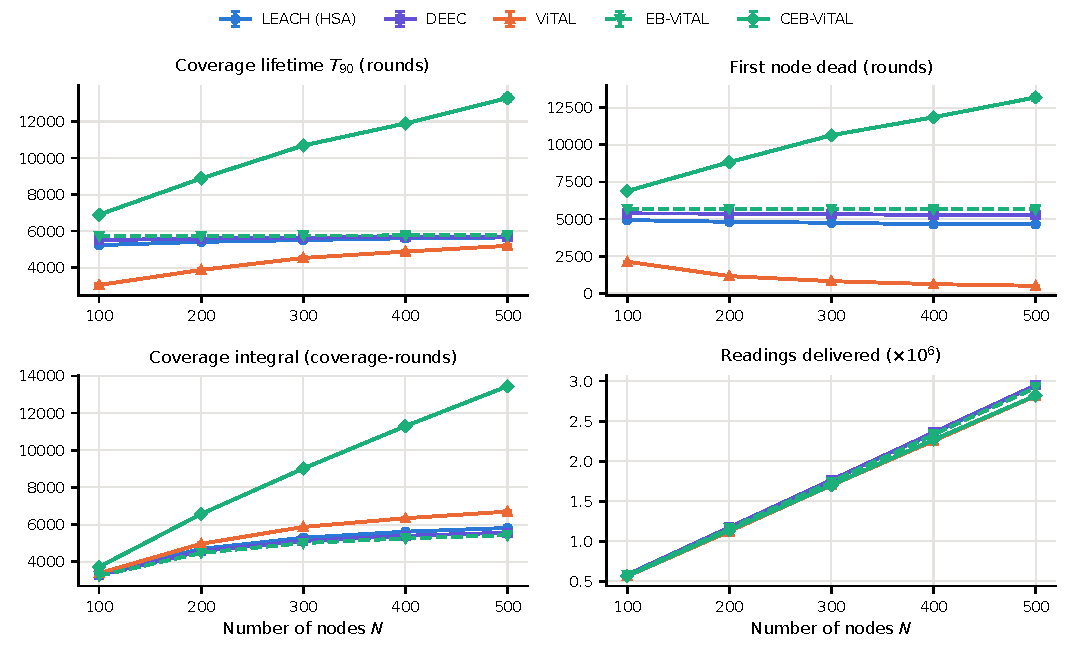
\includegraphics[width=\textwidth]{figures/fig_s1_metrics.pdf}
\caption{Scenario S1: coverage lifetime $\TN$, first node dead, coverage integral and readings delivered versus $N$ (mean $\pm$ 95\% CI).}\label{fig:s1}
\end{figure*}

\begin{table}[t]
\caption{Pre-registered hypotheses in S1. One-sided paired Wilcoxon test with Holm correction over 20 tests per hypothesis.}\label{tab:hyp}
\centering\scriptsize
\begin{tabular}{llccc}
\toprule
Hyp. & Comparator & Gain ($N$=100--500) & Max.\ Holm $p$ & Sig. \\
\midrule
H1 & LEACH (HSA) & +32\% to +135\% & $5.2\times10^{-6}$ & 5/5 \\
 & DEEC & +25\% to +134\% & $5.2\times10^{-6}$ & 5/5 \\
 & ViTAL & +126\% to +156\% & $5.2\times10^{-6}$ & 5/5 \\
 & EB-ViTAL & +21\% to +130\% & $5.2\times10^{-6}$ & 5/5 \\
\midrule
H2 & LEACH (HSA) & +11\% to +131\% & $1.9\times10^{-8}$ & 5/5 \\
 & DEEC & +13\% to +142\% & $1.9\times10^{-8}$ & 5/5 \\
 & ViTAL & +10\% to +101\% & $1.9\times10^{-8}$ & 5/5 \\
 & EB-ViTAL & +15\% to +148\% & $1.9\times10^{-8}$ & 5/5 \\
\midrule
H3 & LEACH (HSA) & +40\% to +184\% & $6.1\times10^{-6}$ & 5/5 \\
 & DEEC & +28\% to +151\% & $6.1\times10^{-6}$ & 5/5 \\
 & ViTAL & +224\% to +2519\% & $6.1\times10^{-6}$ & 5/5 \\
 & EB-ViTAL & +21\% to +134\% & $6.1\times10^{-6}$ & 5/5 \\
\bottomrule
\end{tabular}

\end{table}

\begin{figure}[t]
\centering
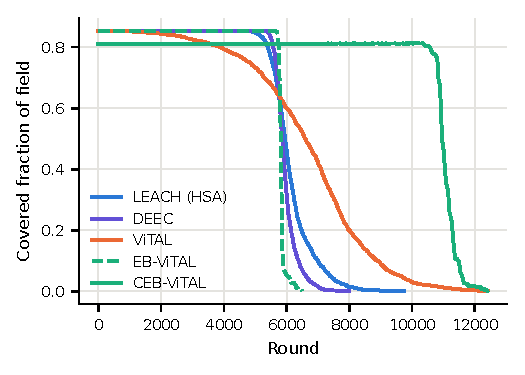
\includegraphics[width=\columnwidth]{figures/fig_cov_time.pdf}
\caption{Covered fraction of the field over time in S1, $N=300$ (mean of 10 networks).}\label{fig:covtime}
\end{figure}

\begin{figure*}[t]
\centering
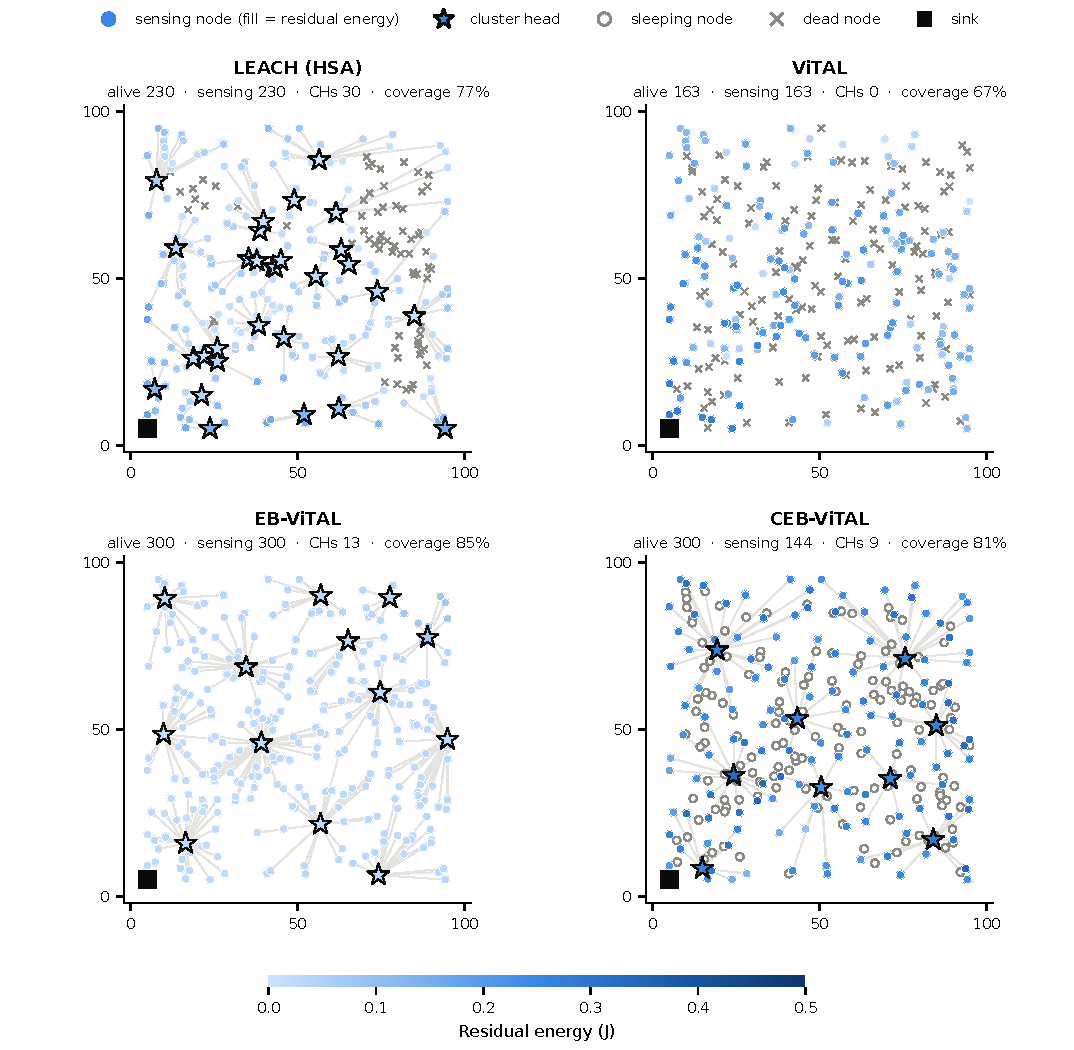
\includegraphics[width=0.86\textwidth]{figures/fig_snapshot.pdf}
\caption{Network state at round \SnapRound{} for one held-out network (S1, $N=\SnapN{}$). Node fill shows residual energy; stars are CHs, hollow circles are sleeping nodes, crosses are dead nodes, and grey lines join members to their CH.}\label{fig:snapshot}
\end{figure*}

\begin{figure*}[t]
\centering
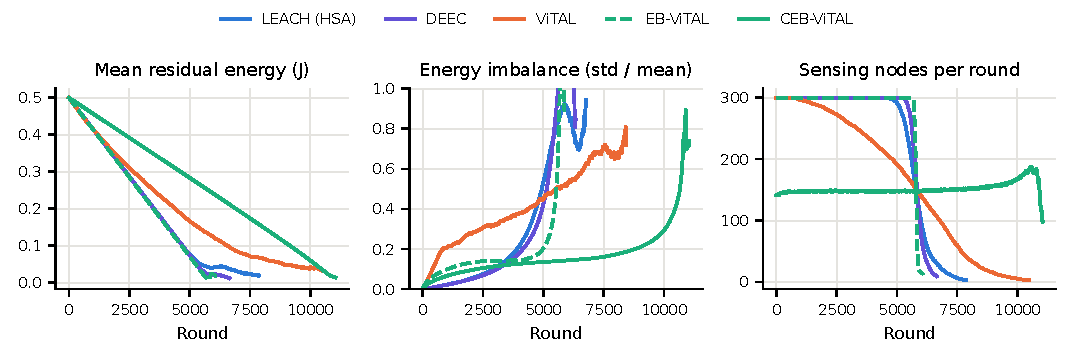
\includegraphics[width=\textwidth]{figures/fig_dynamics.pdf}
\caption{Network dynamics in S1, $N=300$ (mean of 10 held-out networks): mean residual energy of alive nodes, energy imbalance (standard deviation over mean, shown while at least 10\% of nodes are alive), and number of sensing nodes per round.}\label{fig:dynamics}
\end{figure*}

\subsection{Other scenarios}
Table~\ref{tab:cross} compares CEB-ViTAL with the strongest always-on protocol in each scenario. Fig.~\ref{fig:heat} summarises the $\TN$ gain, which ranges from \HeatMin{} to \HeatMax{}, and Fig.~\ref{fig:s3} shows the 200\,m corner-sink field.

\begin{figure*}[t]
\centering
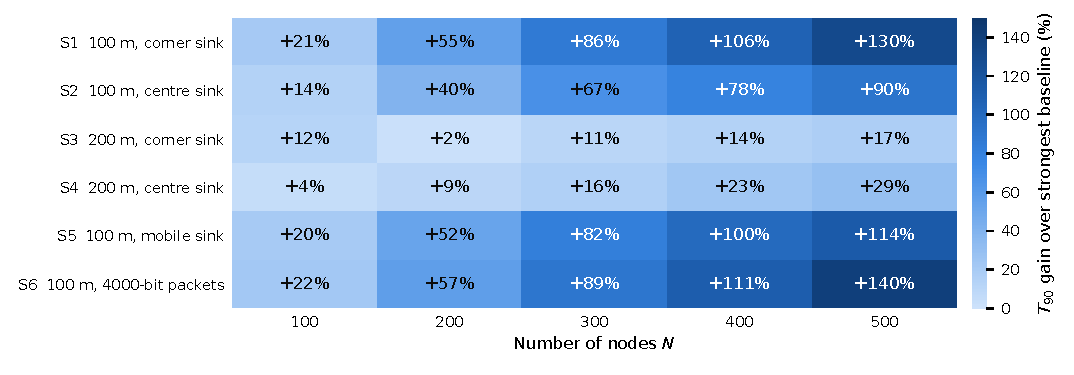
\includegraphics[width=\textwidth]{figures/fig_gain_heatmap.pdf}
\caption{$\TN$ gain of CEB-ViTAL over the strongest always-on protocol for every scenario and network size (mean over 30 held-out networks).}\label{fig:heat}
\end{figure*}

Gains depend on how much redundant coverage the deployment offers. In S3 the $\TN$ gain is only \SthreeTninety{}, because 100 nodes cover just \CzeroSthree{} of a $200\,$m field. In S1, by comparison, 100 nodes cover \CzeroSoneHundred{} and 500 nodes cover \CzeroSoneFive{}.

The mobile sink (S5) and larger packets (S6) reproduce the S1 pattern.

\begin{table*}[t]
\caption{CEB-ViTAL versus the strongest always-on protocol (highest mean $\TN$ among LEACH (HSA), DEEC, ViTAL and EB-ViTAL) in every scenario. Relative change in the mean over 30 held-out networks.}\label{tab:cross}
\centering\footnotesize
\begin{tabular}{cclrrrrr}
\toprule
Scen. & $N$ & Strongest baseline & $T_{90}$ & FND & Cov.\ int. & LND & Readings \\
\midrule
S1 & 100 & EB-ViTAL & +21\% & +21\% & +15\% & +21\% & $-$1\% \\
 & 300 & EB-ViTAL & +86\% & +88\% & +80\% & +89\% & $-$2\% \\
 & 500 & EB-ViTAL & +130\% & +134\% & +148\% & +143\% & $-$3\% \\
\midrule
S2 & 100 & EB-ViTAL & +14\% & +17\% & +11\% & +7\% & $-$1\% \\
 & 300 & ViTAL & +67\% & +696\% & +27\% & +24\% & $-$15\% \\
 & 500 & ViTAL & +90\% & +1561\% & +68\% & +75\% & $-$16\% \\
\midrule
S3 & 100 & EB-ViTAL & +12\% & +141\% & 0\% & +1\% & $-$1\% \\
 & 300 & EB-ViTAL & +11\% & +184\% & +9\% & +11\% & $-$1\% \\
 & 500 & EB-ViTAL & +17\% & +251\% & +20\% & +18\% & $-$1\% \\
\midrule
S4 & 100 & EB-ViTAL & +4\% & +7\% & 0\% & +5\% & $-$2\% \\
 & 300 & EB-ViTAL & +16\% & +18\% & +11\% & +19\% & $-$3\% \\
 & 500 & EB-ViTAL & +29\% & +30\% & +24\% & +37\% & $-$3\% \\
\midrule
S5 & 100 & EB-ViTAL & +20\% & +20\% & +15\% & +24\% & $-$1\% \\
 & 300 & DEEC & +82\% & +89\% & +76\% & +93\% & $-$2\% \\
 & 500 & ViTAL & +114\% & +2036\% & +82\% & +66\% & $-$9\% \\
\midrule
S6 & 100 & EB-ViTAL & +22\% & +22\% & +16\% & +22\% & 0\% \\
 & 300 & EB-ViTAL & +89\% & +91\% & +82\% & +92\% & $-$1\% \\
 & 500 & EB-ViTAL & +140\% & +141\% & +148\% & +147\% & $-$1\% \\
\bottomrule
\end{tabular}

\end{table*}

\begin{figure*}[t]
\centering
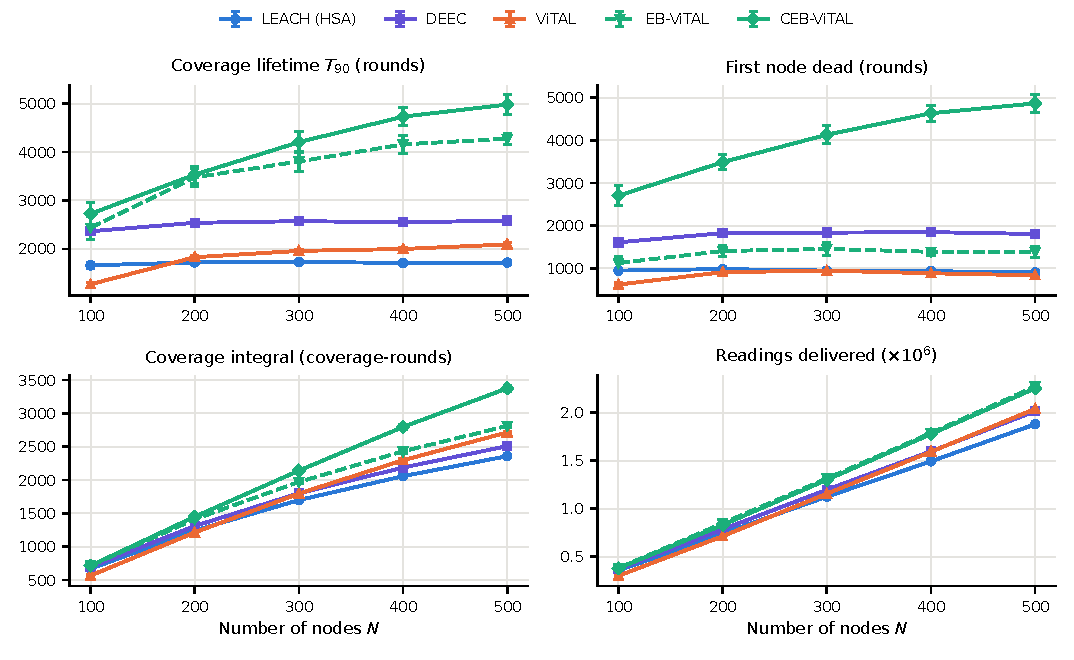
\includegraphics[width=\textwidth]{figures/fig_s3_metrics.pdf}
\caption{Scenario S3 (200\,m field, sink at (5,5)).}\label{fig:s3}
\end{figure*}

\subsection{Ablation}
Table~\ref{tab:abl} isolates each component.
\begin{itemize}
\item \textbf{Scheduling vs.\ clustering.} Both phases matter. In the 100\,m field, removing CovSched costs more than replacing the clustering for $N\ge200$; at $N=100$ the two are comparable. In the sparse 200\,m field (S3), the EB clustering contributes more than the scheduler.
\item \textbf{Node selection.} Choosing the same number of sleepers at random drops coverage below $0.9C_0$ within the first rounds in all but the sparsest settings, so selection matters as much as the number of active nodes.
\item \textbf{Clustering.} Replacing EB clustering with LEACH under the same scheduler lowers $\TN$; CEB-ViTAL is \LeachCovSone{} better in S1.
\item \textbf{Multi-hop forwarding (M3).} It has no measurable effect in the $100\,$m fields, where relays are rarely cheaper than direct links. In S3 its effect is \MthreeSthree{}.
\end{itemize}

\begin{table*}[t]
\caption{Ablation: change in CEB-ViTAL relative to each variant, shown as $\TN$ / FND / coverage integral. $^\dagger$The variant's mean $\TN$ is below 100 rounds, so a ratio is not meaningful.}\label{tab:abl}
\centering\footnotesize
\begin{tabular}{cl ccc}
\toprule
Scen. & Variant & $N{=}100$ & $N{=}300$ & $N{=}500$ \\
\midrule
S1 & No CovSched (always on) & +21\% / +21\% / +15\% & +86\% / +88\% / +80\% & +130\% / +134\% / +148\% \\
 & Random sleepers, same count & $\approx$0$^\dagger$ / $-$1\% / +10\% & $\approx$0$^\dagger$ / $-$9\% / +17\% & $\approx$0$^\dagger$ / $-$26\% / +12\% \\
 & LEACH clustering instead of EB & +23\% / +23\% / +6\% & +61\% / +61\% / +23\% & +58\% / +59\% / +25\% \\
 & No multi-hop (M3) & 0\% / 0\% / 0\% & 0\% / 0\% / 0\% & 0\% / 0\% / 0\% \\
\midrule
S3 & No CovSched (always on) & +12\% / +141\% / 0\% & +11\% / +184\% / +9\% & +17\% / +251\% / +20\% \\
 & Random sleepers, same count & +35\% / +129\% / +1\% & $\approx$0$^\dagger$ / +137\% / +7\% & $\approx$0$^\dagger$ / +146\% / +10\% \\
 & LEACH clustering instead of EB & +41\% / +41\% / +8\% & +110\% / +108\% / +24\% & +140\% / +138\% / +36\% \\
 & No multi-hop (M3) & +3\% / +3\% / +3\% & 0\% / +1\% / +2\% & +2\% / +4\% / +3\% \\
\bottomrule
\end{tabular}

\end{table*}

\subsection{Robustness to sleep energy}
The radio model treats sleeping as free. We therefore added a check that was \emph{not} pre-registered: every sleeping node is charged $f L E_{\mathrm{elec}}$ per round. With $f=1$, sleeping costs as much as the electronics energy of sending one packet. This penalises only the scheduled protocols.

Table~\ref{tab:rob} shows the results.
\begin{itemize}
\item In S1, CEB-ViTAL keeps a positive $\TN$ advantage even at $f=1$ (\RobSoneFone{}).
\item In the sparse S3 field, the $\TN$ advantage disappears at $f=1$ (\RobSthreeFone{}), although FND remains much longer.
\end{itemize}

\begin{table*}[t]
\caption{Sleep-energy robustness (post hoc). CEB-ViTAL versus the strongest always-on protocol, shown as $\TN$ / FND / coverage integral.}\label{tab:rob}
\centering\footnotesize
\begin{tabular}{cc cccc}
\toprule
Scen. & $N$ & $f=0$ & $f=0.05$ & $f=0.25$ & $f=1$ \\
\midrule
S1 & 100 & +21\% / +21\% / +15\% & +20\% / +21\% / +14\% & +18\% / +18\% / +12\% & +10\% / +10\% / +4\% \\
 & 300 & +86\% / +88\% / +80\% & +83\% / +86\% / +78\% & +75\% / +75\% / +66\% & +37\% / +35\% / +28\% \\
 & 500 & +130\% / +134\% / +148\% & +125\% / +128\% / +141\% & +108\% / +105\% / +115\% & +56\% / +49\% / +45\% \\
\midrule
S3 & 100 & +12\% / +141\% / 0\% & +11\% / +140\% / 0\% & +10\% / +137\% / 0\% & +6\% / +129\% / $-$1\% \\
 & 300 & +11\% / +184\% / +9\% & +10\% / +182\% / +9\% & +6\% / +174\% / +7\% & $-$3\% / +144\% / +3\% \\
 & 500 & +17\% / +251\% / +20\% & +15\% / +248\% / +20\% & +10\% / +234\% / +17\% & 0\% / +157\% / +9\% \\
\bottomrule
\end{tabular}

\end{table*}

\section{Discussion and Threats to Validity}\label{sec:threats}
\textbf{Coverage level.} CEB-ViTAL trades a fixed share of instantaneous coverage ($1-\tau=5\%$) for a much longer coverage lifetime. Applications that need every coverable cell at every instant should raise $\tau$ or use an always-on protocol.

\textbf{ViTAL baseline.} ViTAL is our re-implementation from its paper. Several of its parameters are not published, including $E_{\mathrm{elec}}$, $p$, the weights $w_1$--$w_4$ and the SNR model. Our absolute ViTAL numbers therefore differ from those reported in~\cite{ali2025vital}, and comparisons with ViTAL should be read with that caveat. LEACH and DEEC are fully specified.

\textbf{Model scope.} The study uses the first-order radio model, with no packet loss, MAC contention or idle listening, and data links are not limited by radio range, as in LEACH-type studies. The sleep-energy check bounds one of these simplifications.

\textbf{Centralised control.} The scheduler and the election run at the sink, as in LEACH-C and ViTAL.

\textbf{Constants.} The constants $\tau$, $r_s$, $L_{\mathrm{ctrl}}$ and the M1 weight schedule were fixed before testing and not tuned. Other values may perform better or worse.

\section{Conclusion}
Coupling ViTAL's coverage-driven deployment with coverage-preserving, energy-weighted sleep scheduling and corrected, energy-balanced clustering substantially extends coverage lifetime in dense networks, with only a small change in delivered readings. Future work includes distributed scheduling, validation against the original ViTAL implementation, packet-level simulation and a hardware testbed.

\clearpage
\section*{Data and Code Availability}
The simulator, the pre-registration, the raw run data (\NRuns{} test runs and \NRob{} robustness runs) and the analysis scripts will be released at \todo{repository URL}. Every number in this paper is generated from those data by the released scripts.

\section*{Declaration on the Use of AI Tools}
\todo{Authors: state how AI tools were used in coding, analysis and writing, as required by the target journal's policy, and confirm that you have verified all content.}

\section*{Author Contributions}
\todo{Authors: state each author's contribution, e.g.\ using the CRediT taxonomy.}

\bibliographystyle{IEEEtran}
\bibliography{refs}

\end{document}
